%% LyX 2.2.3 created this file.  For more info, see http://www.lyx.org/.
%% Do not edit unless you really know what you are doing.
\documentclass[english]{article}
\usepackage[T1]{fontenc}
\usepackage[latin9]{inputenc}
\usepackage{geometry}
\geometry{verbose,tmargin=2cm,bmargin=2cm,lmargin=2cm,rmargin=2cm}
\setlength{\parskip}{\medskipamount}
\setlength{\parindent}{0pt}
\usepackage{xcolor}
\usepackage{babel}
\usepackage{graphicx}
\usepackage[unicode=true]
 {hyperref}
\usepackage{breakurl}

\makeatletter
%%%%%%%%%%%%%%%%%%%%%%%%%%%%%% User specified LaTeX commands.
% Added by lyx2lyx
\@ifundefined{rangeHsb}{\usepackage{xcolor}}{}

\makeatother

\begin{document}

\title{The (GRIM)REEPER}

\author{Ken Livingston}
\maketitle
\begin{center}
(\textbf{\textcolor{purple}{G}}RIM \textbf{\textcolor{purple}{R}}EEPER\textbf{
}\textbf{\textcolor{purple}{I}}mplements \textbf{\textcolor{purple}{M}}acros
to) \textbf{\textcolor{purple}{R}}ead \textbf{\textcolor{purple}{E}}PICS
\textbf{\textcolor{purple}{E}}vents and \textbf{\textcolor{purple}{P}}lot
\textbf{\textcolor{purple}{E}}verything in \textbf{\textcolor{purple}{R}}OOT
\par\end{center}

\begin{center}
\begin{figure}[h]
\centering{}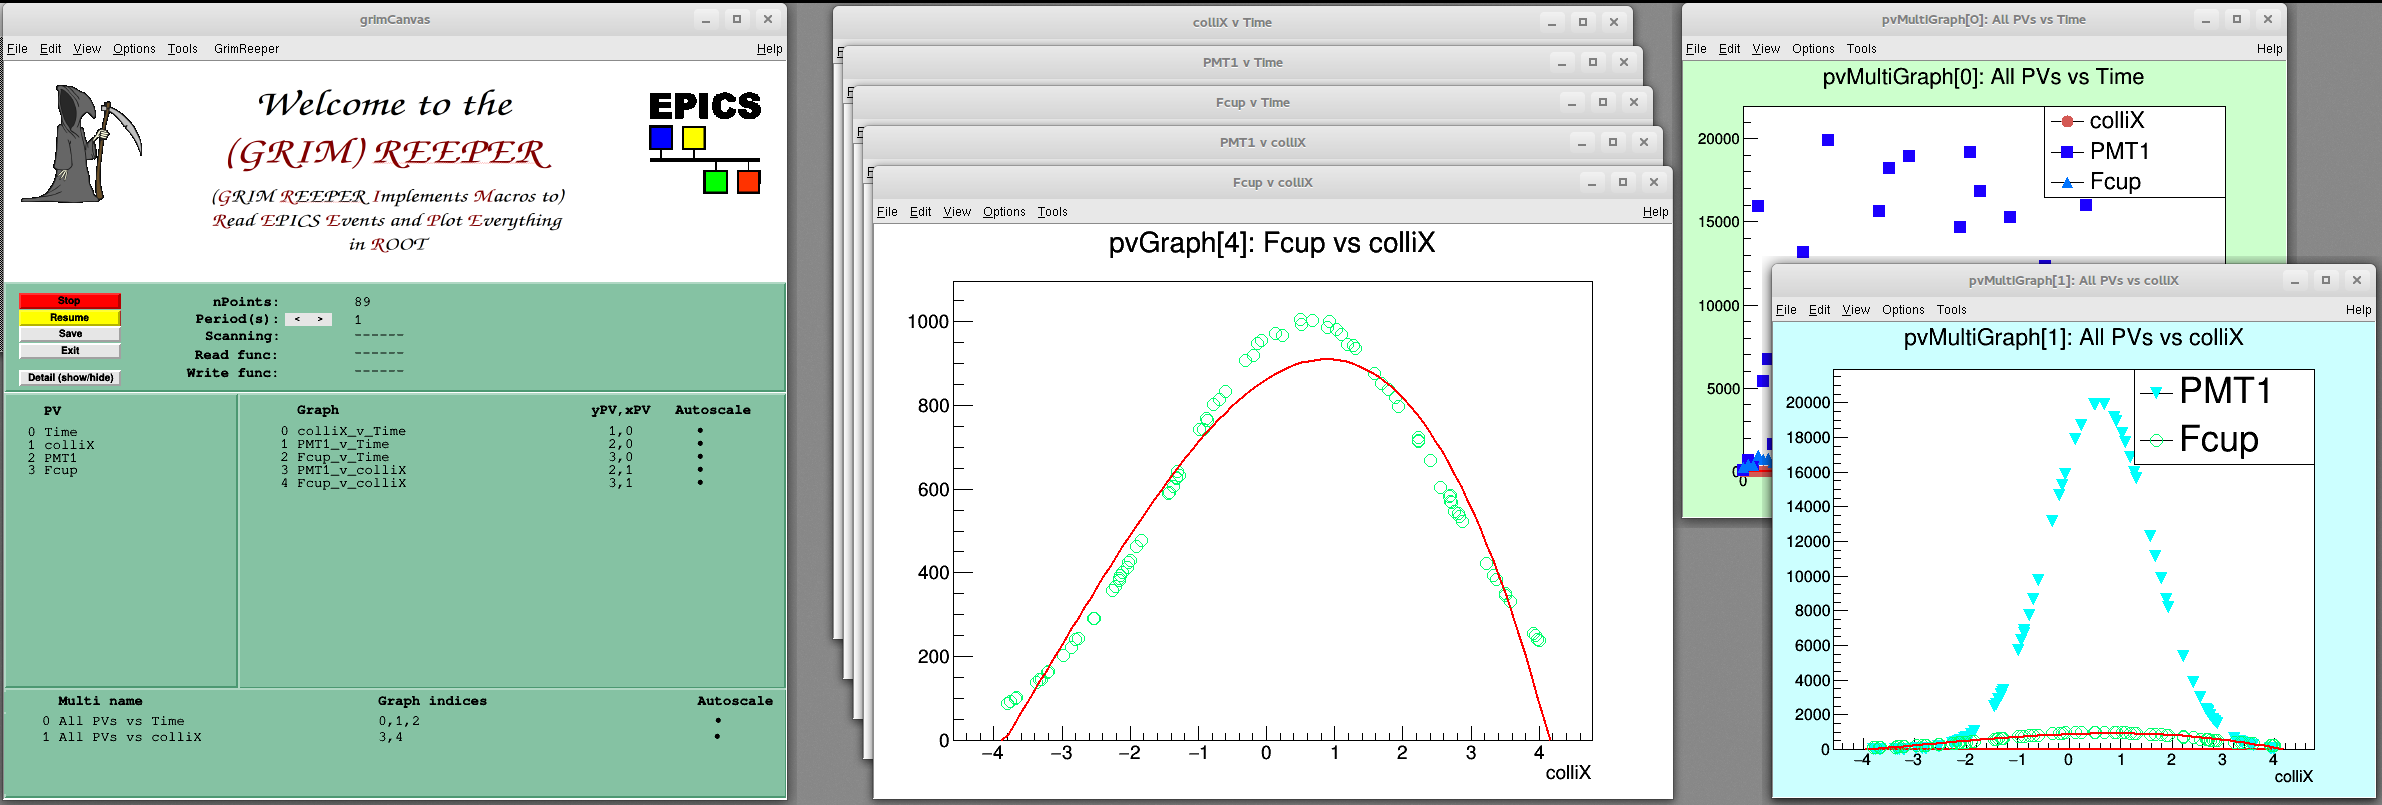
\includegraphics[width=0.8\paperwidth]{allthings}\caption{\label{fig:GrimReeper-windows}REEPER windows}
\end{figure}
\par\end{center}

\section{Overview}

(GRIM)REEPER, is a package for plotting EPICS PVs (Process Variables)
in ROOT. At it's simplest it can be used as a strip chart, and, at
it's most complex, as a general tool for modifying one or more EPICS
PVs in a scan, reading back many PVs and analysing the result. The
display (Figure \ref{fig:GrimReeper-windows}) consists of one or
more of the following:

\textbf{Status and control window} (left). This is optional. \textbf{}\\
\textbf{Graphs} (middle). One or more canvases, each with a graph
of a PV vs Time, or PVy vs PVx.\textbf{}\\
\textbf{MultiGraphs} (Right). Showing one or more graphs on the same
canvas.

It runs with a command line utility which has 2 modes:\texttt{ }

\texttt{\footnotesize{}reeper {[}OPTION{]}... {[}PV1{]} {[}PV2{]}
... ~~~~~~~~~~~~~~~~~~~~~~~~~~~~~~~~~~~~~~~~~}\texttt{\textcolor{purple}{\footnotesize{}\textbackslash{}\textbackslash{}mode1}}\texttt{\footnotesize{}}~\\
\texttt{\footnotesize{}reeper {[}ROOT OPTIONS{]}...{[}file1.C{]} ... fileN.C{]}
~~~~~~~~~~~~~~~~~~~~~~~~~~~~~}\texttt{\textcolor{purple}{\footnotesize{}\textbackslash{}\textbackslash{}mode2}}\texttt{\footnotesize{}}~\\
\texttt{ }

\textbf{mode1} is for specification of PVs, scan parameters, fit fuctions
etc to set up periodic reading of PVs and plotting of graphs and multiGraphs.
The use of the \texttt{\footnotesize{}-w <start, stop, step>} option
writes an updated value to PV1 before each time period (with caput
commands). 

\textbf{mode2} is for customization using ROOT macros to call the
REEPER functions directly. 

Examples are given in Section \ref{sec:Quickstart} and full documentation
in section \ref{sec:Detailed-documentation}.

\section{\label{sec:Quickstart}Quickstart}

\subsection*{Prequisites}

You must be running on a system with a working ROOT installation,
EPICS channel access and \texttt{\footnotesize{}caget, caput} in your
path\textcolor{black}{{} (and }\texttt{\textcolor{black}{\footnotesize{}softIOC}}\textcolor{black}{,
if you want to try the simulated examples)}

\subsection*{Setup}

Source the relevant setup in your\texttt{\textcolor{black}{\footnotesize{}
.cshrc or .bashrc: }}~\\
\texttt{\textcolor{black}{\footnotesize{}source <reeper\_installation>/thisreeper.csh
or <reeper\_installation>/thisreeper.sh}}{\footnotesize \par}

This sets the environment variable \texttt{\footnotesize{}\$REEPER}
to point to the installation directory, and adds it to the \texttt{\footnotesize{}\$PATH}{\footnotesize \par}

\subsection*{Examples 1 - specifying PVs on the command line.}

These examples use simulation mode (\texttt{\footnotesize{}-s} flag)
which runs a softIOC. The \texttt{\footnotesize{}Exit} button on the
control panel will kill the \texttt{\footnotesize{}softIOC} process
before quitting ROOT, otherwise it may need to be killed manually,
later. The status and control window is not shown, since it is common
to all, and is documented in more detail below.The examples get progressively
more fancy.
\begin{itemize}
\item Several different examples of specifying a single PV for plotting
(Figure \ref{fig:Five-different-ways})\texttt{}~\\
\texttt{\footnotesize{}>reeper -s colliX ~~~~~~~~~~~~~~~~~~~~~~~~~~~~~~~~~~~~~\textcolor{purple}{//plot
colliX vs Time }}~\\
\texttt{\footnotesize{}>reeper -s colliX::L~~~~~~~~~~~~~~~~~~~~~~~~~~~~~~~~~~~\textcolor{purple}{//plot
colliX vs time, join with line} }~\\
\texttt{\footnotesize{}>reeper -s colliX::C~~~~~~~~~~~~~~~~~~~~~~~~~~~~~~~~~~~\textcolor{purple}{//plot
colliX vs time, join with curve}}~\\
\texttt{\footnotesize{}>reeper -s colliX::pol3~~~~~~~~~~~~~~~~~~~~~~~~~~~~~~~~\textcolor{purple}{//plot
colliX vs time, fit with pol3}}~\\
\texttt{\footnotesize{}>reeper -s colliX::pol3,10,20~~~~~~~~~~~~~~~~~~~~~~~~~~\textcolor{purple}{//plot
colliX vs time, fit with pol3 in range 10-20s}}\\
\begin{figure}[h]
\centering{}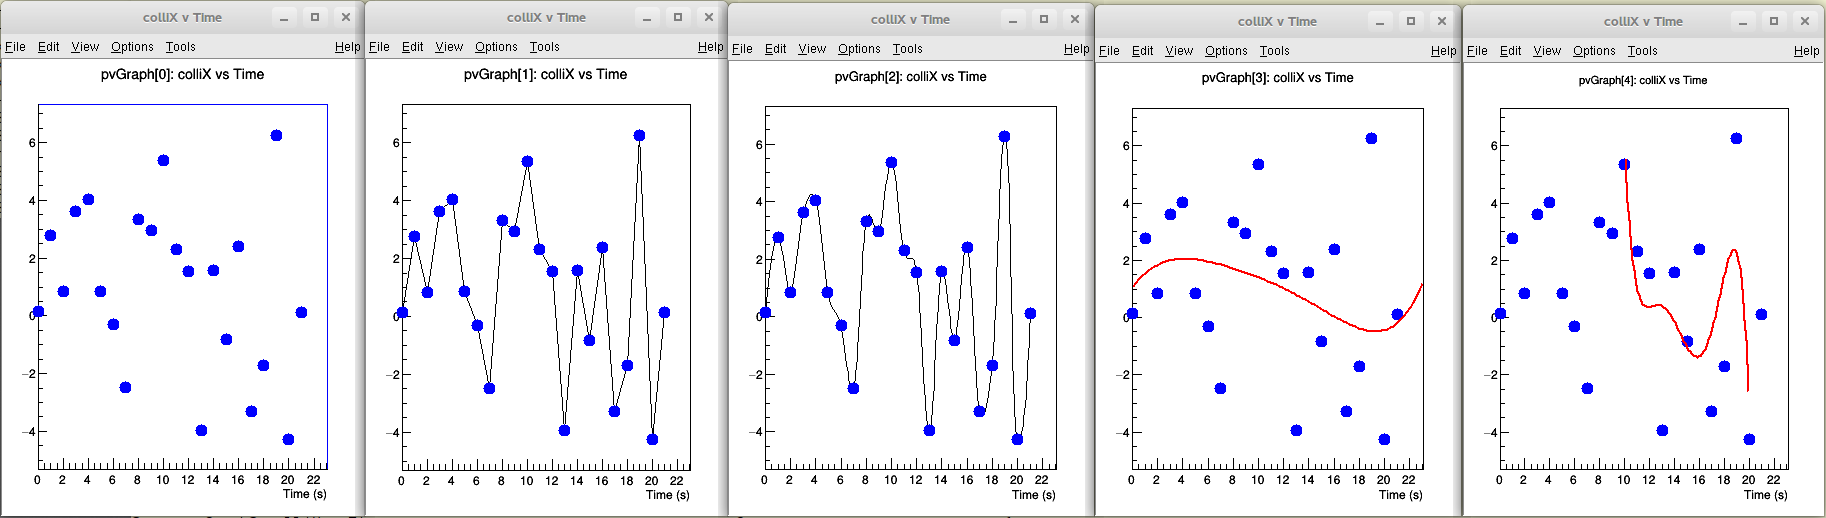
\includegraphics[width=0.8\paperwidth]{fiveways}\caption{\label{fig:Five-different-ways}Several ways of plotting the graph
of a PV using the command line tool}
\end{figure}
\item Multiple PVs can be specified on the command line, with the option
of writing (\texttt{\footnotesize{}caput}) to PV1 to do a scan (Figure
\ref{fig:example2})\textcolor{white}{{} }
\item \texttt{\footnotesize{}>reeper -s -x colliX::pol3 PMT1\#\#gaus,-4,4
Fcup\#\#pol3 ~~\textcolor{purple}{//All PVs vs Time and PMT1, Fcup
vs colliX, with fits } }~\\
\texttt{\footnotesize{}>reeper -s -w -4,4,0.1 colliX::pol3 PMT1\#\#gaus,-4,4
Fcup\#\#pol3~~\textcolor{purple}{//As above, but scan from -4 to
+4 in colliX} }\texttt{}~\\
\texttt{}~\\
The\texttt{\footnotesize{} -x} option causes the creation of an extra
set of graphs where all PVs are plotted vs PV1. \\
The \texttt{\footnotesize{}-w {[}start,stop,step{]}} option causes
the same behaviour, but actively controls PV1 (colliX) using \texttt{\footnotesize{}caput}
commands. \\
For the PVs where a fit is specified, the \texttt{\footnotesize{}::}
delimiter means the fit is applied to the Time graph, and the \texttt{\footnotesize{}\#\#}
delimiter means it is applied to the PV1 graph. Two multiGraphs are
also produced - one with all the Time graphs and one with all the
PV1 graphs. The axes on all graphs will autoscale, by default, each
time a new point is added unless autoscaling it turned off (\emph{toggle
autoscaling} on the context menu on the graph's canvas using the RH
mouse button). The colours and symbols are changed automatically for
every new graph, in a tasteless and unpredictable manner, but can
be improved by bringing up the editor from the ROOT toolbar.\texttt{}~\\
\begin{figure}[h]
\centering{}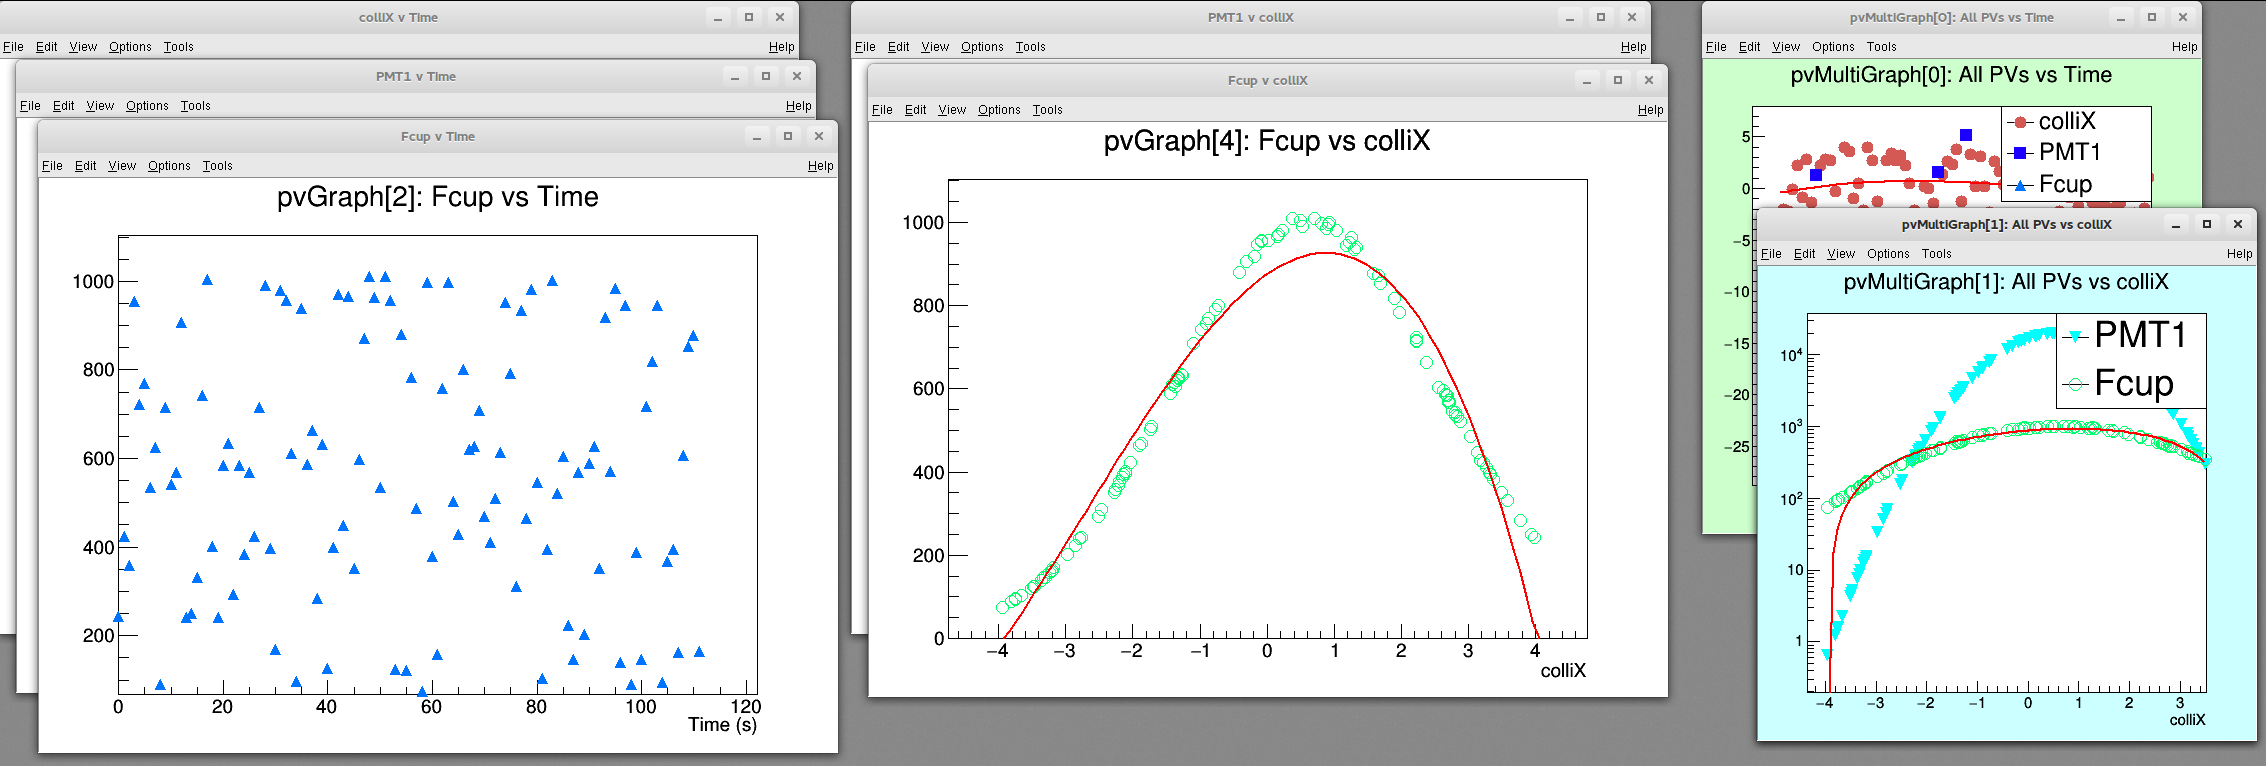
\includegraphics[width=0.8\paperwidth]{example2}\caption{\label{fig:example2}Multiple PVs, some with fits. Graphs and multiGraphs
of all PVs vs Time, and vs PV1 are made }
\end{figure}
\end{itemize}

\subsection*{Examples 2 - specifying PVs in a ROOT macro}
\begin{itemize}
\item The inclusion of one or more \texttt{\footnotesize{}.C} files on the
command line opens ROOT with the REEPER library loaded and processes
arguments in the standard ROOT way. For example:\\
\texttt{\footnotesize{}>reeper grBasic.C ~~~~~~~~~~~~~~~~\textcolor{purple}{//Sets
up a simple scan and plots one PV against another } }~\\
\texttt{\footnotesize{}>reeper grScanFancy.C~~~~~~~~~~~~~\textcolor{purple}{//Shows
how to do a 2d scan, fill 2d histograms and read waveforms } }\\
\\
The files \texttt{\footnotesize{}grBasic.C} and\texttt{\footnotesize{}
grScanFancy.C} are included in the \texttt{\footnotesize{}\$REEPER}
directory. The run using the built in simulation, and are well commented.
They should be used as templates to help write macros to deal with
real PVs.
\end{itemize}
The ROOT prompt is always available and the global variable nd be
used to access the class members functions and data, which are all
public. Yes - plenty of scope for screwing this up! This is all described
in section \ref{sec:Detailed-documentation}.

\section{\label{sec:Detailed-documentation}Detailed documentation}

A brief description with options, arguments and usage, is given by
running \texttt{\footnotesize{}>reeper -h} (see \ref{subsec:reeper--h}).
Some more detail is given here.

REEPER is a collection of functions and variables to do EPICS read/write,
and plot the results. All the functions can be accessed from the ROOT
prompt, or by using a ROOT macro. The command line utility \texttt{\footnotesize{}reeper}
calls a specific set of these commands, then offers the ROOT prompt,
where a knowledgeable user could type commands to generate more graphs,
save canvases etc. Access to some commands is provided via the status
/ control panel, which is created by default when \texttt{\footnotesize{}reeper}
is called, (or can be brought up by calling \texttt{\footnotesize{}makeControlGUI()}
from the ROOT prompt).

The documentation below describes aspects of the functionality in
an \emph{inverse need to know} order (the more obscure and specialised
information comes towards the end).

\subsection{Control / Status Panel and context menu options}

\begin{figure}[h]
\begin{centering}
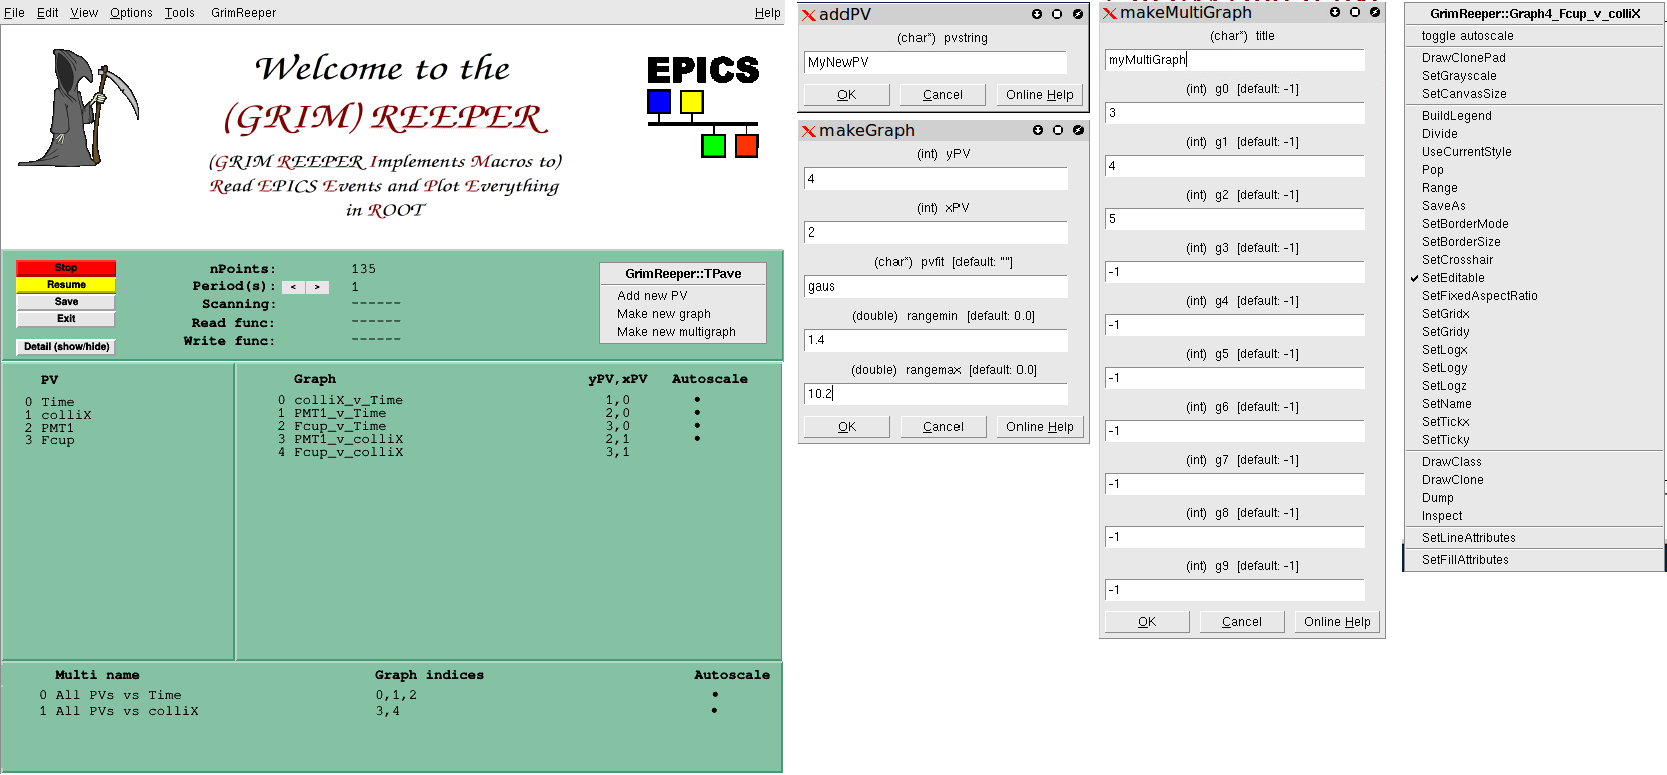
\includegraphics[bb=0bp 0bp 1667bp 770bp,width=0.9\paperwidth]{allguis}\caption{\label{fig:Control-panel-and}Control panel and context menus for
panel and graphs / multiGraph canvases}
\par\end{centering}
\end{figure}

The control panel is shown in Figure \ref{fig:Control-panel-and}
(left):
\begin{itemize}
\item \textbf{Stop, Start, Pause/Resume, Exit.} Do the obvious.
\item \textbf{Save.} Saves the data in several ways:
\begin{itemize}
\item PVs are written a text file with columns. Eg.\\
\texttt{\footnotesize{}\# PV0 = Time }~\\
\texttt{\footnotesize{}\# PV1 = colliX }~\\
\texttt{\footnotesize{}\# PV2 = PMT1 }~\\
\texttt{\footnotesize{}\# PV3 = Fcup }~\\
\texttt{\footnotesize{}\#step PV0 ~~~~PV1 ~~~~~~~PV2 ~~~~~PV3
}~\\
\texttt{\footnotesize{}0 ~~~~0.0000 -2.7656 ~~~69.3981 243.0320
}~\\
\texttt{\footnotesize{}1 ~~~~1.0000 -2.0289 ~~631.3830 423.8440
}~\\
\texttt{\footnotesize{}2 ~~~~2.0000 -2.2597 ~~335.1750 357.4400
}~\\
\texttt{\footnotesize{}3 ~~~~3.0000 -0.0776 15897.6000 953.7850
}~\\
\texttt{\footnotesize{}4 ~~~~4.0000 ~2.2213 ~5373.3400 722.6930
}~\\
\texttt{\footnotesize{}5 ~~~~5.0000 -0.8775 ~6714.0500 768.8300
}~\\
\texttt{\footnotesize{}6 ~~~~6.0000 ~2.8360 ~1642.0800 534.1220
}\\
....\\
....\\
These can then be easily read back into ROOT as graphs (eg. for PV2,
PV3): \texttt{}~\\
\texttt{\footnotesize{}g = new TGraph(\textquotedbl{}file\textquotedbl{},\textquotedbl{}\%{*}s\%{*}s\%{*}s\%lg\%lg\textquotedbl{})}{\footnotesize \par}
\item Graphs are written as \texttt{\footnotesize{}.root, .pdf, .gif }and\texttt{\footnotesize{}
.C} files
\item By default they are written with timestamps like this into directory
\texttt{epics\_gr}, like this: \texttt{}~\\
\texttt{\footnotesize{}epics\_gr/gr\_save\_15\_05\_17-11\_07.txt,
}~\\
\texttt{\footnotesize{}epics\_gr/Graph2\_Fcup\_v\_Time\_15\_05\_17-11\_07.gif
... etc.}{\footnotesize \par}
\item The output directory can be changed that root prompt: \\
\texttt{\footnotesize{}GR->setSaveDir(\textquotedbl{}mydir\textquotedbl{})}{\footnotesize \par}
\item The list of formats can also be changed: eg. \\
\texttt{\footnotesize{}char {*}mySaveFormats{[}{]} = \{\textquotedbl{}C\textquotedbl{},\textquotedbl{}pdf\textquotedbl{},NULL\}}~\\
\texttt{\footnotesize{}GR->setSaveFormats(mySaveFormats)}{\footnotesize \par}
\end{itemize}
\item \textbf{nPoints}. Number of read events in the scan.
\item \textbf{Period}. Time (s) between read. Can be changed with the arrows
in increments of 1s.
\item \textbf{Scanning}. If a PV is being controlled with caput commands,
start,stop,step and current value are shown.
\item \textbf{Read / Write func}. Details of user defined read/write functions.
\item \textbf{Details}. This buttons toggles the visibility of the bottom
half of the GUI, which shows the current lists of PVs, graphs and
mulitGraphs.
\end{itemize}

\subsubsection*{Context Menus}

Some useful REEPER functions are available via ROOT context menus
(Figure \ref{fig:Control-panel-and} (right)). Context menus are brought
up by clicking the right mouse button over an item; the options depend
on the context (ie the entity over which the mouse was hovering when
clicked). 
\begin{itemize}
\item \textbf{Control panel context menu}. This is the \texttt{GrimReeper::TPave}
menu, shown on top right of the green zone in Figure \ref{fig:Control-panel-and}
(left). The 3 options each pop up a different input dialog box (also
shown in the figure). They are simply calling functions that are part
of REEPER, and could also be typed at the ROOT prompt:
\begin{itemize}
\item \textbf{addPV}: Add a new PV. If this is mid scan, points relating
to earlier time steps are set to zero for this PV. The new PV now
becomes available for making graphs.
\item \textbf{makeGraph}: Create a graph from any 2 PVs specified by index.
PV0 is always Time. There is the option to include a fit and range
as illustrated in Section \ref{sec:Quickstart}.
\item \textbf{makeMultiGraph}: Create a multiGraph from several graphs,
specified by index. The x axis will be taken from the 1st graph.
\end{itemize}
\item \textbf{Graph Canvas context menu}. This is the standard Graph canvas
with an added option at the top:
\begin{itemize}
\item \textbf{toggle autoscale}. This toggles the autoscaling on/off for
the relevant graph or multiGraph. When autoscaling is on it will be
applied every time the graph is redrawn with new data. The status
of autoscaling can be seen in the bottom part of the control GUI.
\end{itemize}
\end{itemize}

\subsection{Concepts, coding approach etc}

In a counting house, EPICS experts might do quick PV scans using a
combination of unix shell tools (sh, awk etc), piping the output to
text files and opening ROOT to make any required graphs and fit the
data. The grimReeper is an attempt to make that easier - particularly
for users with limited ROOT and unix experience. The main design features
are:
\begin{itemize}
\item \textbf{PV0 = Time}: The fundamental PV for the grimReeper is Time.
PV0 is always Time(s), and scanning is done in time steps.
\item \textbf{Command line use}: Basic behaviour is accessible with a simple
shell command in the standard unix style. \\
\texttt{reeper} is a shell(sh) script which parses args and opts and
opens ROOT as required. 
\item \textbf{ROOT}: Once ROOT is opened, all standard functionality is
available at the ROOT prompt; the global variable \texttt{\footnotesize{}grimReeper
{*}GR}, allows control of scanning, visuals, etc and gives access
to the raw PV data. GUI features are an \emph{add-on}. 
\item \textbf{GUI}: Fancy ROOT GUIs are too complicated to produce and need
lots of code. The simple GUI functionality here is using \texttt{\footnotesize{}TButton}
and customization of \texttt{\footnotesize{}TContextMenu} items.
\item \textbf{Compilation}: This is done \emph{on the fly}, using ROOT's
ACLiC features. No makefiles. The details can be seen in \texttt{\footnotesize{}reeper}
and \texttt{\footnotesize{}grLoad.C}. Debugging can be done with gdb
if required\\
For example, see \href{https://wiki.physik.uni-muenchen.de/etp/index.php/Debugging_root_with_gdb}{https://wiki.physik.uni-muenchen.de/etp/index.php/Debugging\_{}root\_{}with\_{}gdb}.
\end{itemize}

\subsection{\texttt{Class grimReeper}}

The grimReeper class definition is in \texttt{\footnotesize{}gr.C},
which also defines a global variable \texttt{\footnotesize{}grimReeper
{*}GR} pointing to the (single) grimReeper object. This allows the
member functions to be accessed from the commend line and from \texttt{\textcolor{black}{\footnotesize{}TButtons}}.
For details look into the code. Everything is public, so lots of opportunity
to mess things up! Some functions are worth a special mention, since
they are useful for macros:

\texttt{\footnotesize{}void setMAXPV(int maxpv) ~~~~~~~~~~~~~~~~}\texttt{\textcolor{purple}{\footnotesize{}\textbackslash{}\textbackslash{}set
max no of PVs that can be added (default = 50)}}\texttt{\footnotesize{}}~\\
\texttt{\footnotesize{}void setMAXDATA(int data)~~~~~~~~~~~~~~~~}\texttt{\textcolor{purple}{\footnotesize{}\textbackslash{}\textbackslash{}set
max no of read points per PV (default = 10000)}}\texttt{\footnotesize{}}~\\
\texttt{\footnotesize{}Note: The above functions must be called before
init()}~\\
\texttt{\footnotesize{}void intit();~~~~~~~~~~~~~~~~~~~~~~~~~~~~}\texttt{\textcolor{purple}{\footnotesize{}\textbackslash{}\textbackslash{}set
up initial params, arrays etc. This is called implicitly ny addPV()}}\texttt{\footnotesize{}}~\\
\texttt{\footnotesize{}void addPV(const char {*}pvstring);~~~~~~~~}\texttt{\textcolor{purple}{\footnotesize{}\textbackslash{}\textbackslash{}add
PV to the list being read (each call adds 8{*}MAXDATA bytes to memory
used)}}\texttt{\footnotesize{}}~\\
\texttt{\footnotesize{}void makeGraph(int yPV, int xPV, ...);~~~}\texttt{\textcolor{purple}{\footnotesize{}\textbackslash{}\textbackslash{}add
new graph (each will require memory dynamically up to 16{*}MAXDATA
bytes)}}\texttt{\footnotesize{}}~\\
\texttt{\footnotesize{}int getPoints() ~~~~~~~~~~~~~~~~~~~~~~~~~}\texttt{\textcolor{purple}{\footnotesize{}\textbackslash{}\textbackslash{}number
of PV scan points read so far}}\texttt{\footnotesize{}}~\\
\texttt{\footnotesize{}double {*}{*}getPVData()~~~~~~~~~~~~~~~~~~~~~}\texttt{\textcolor{purple}{\footnotesize{}\textbackslash{}\textbackslash{}2d
array of PV data: array{[}PVindex{]}{[}point{]}}}\texttt{\footnotesize{}}~\\
\texttt{\footnotesize{}void setUserWrite(const char {*}write)~~~~~}\texttt{\textcolor{purple}{\footnotesize{}\textbackslash{}\textbackslash{}user
function to be called to write PVs for a step}}\texttt{\footnotesize{}}~\\
\texttt{\footnotesize{}void setUserRead(const char {*}read)~~~~~~~}\texttt{\textcolor{purple}{\footnotesize{}\textbackslash{}\textbackslash{}user
function to be called after scan step period elapsed}}\texttt{\footnotesize{}}~\\
\texttt{\footnotesize{}void waveToArray(const char {*}pv, ...);~~~}\texttt{\textcolor{purple}{\footnotesize{}\textbackslash{}\textbackslash{}read
waveform into arrray}}\texttt{\footnotesize{}}~\\
\texttt{\footnotesize{}void waveToTH1D(const char {*}pv,...);~~~~~}\texttt{\textcolor{purple}{\footnotesize{}\textbackslash{}\textbackslash{}read
waveform into 1D histogram bins 1D}}\texttt{\footnotesize{}}~\\
\texttt{\footnotesize{}void waveToTH2DRow(const char {*}pv,...);~~}\texttt{\textcolor{purple}{\footnotesize{}\textbackslash{}\textbackslash{}read
waveform into a row of a 2D histogram}}{\footnotesize \par}

The use is discussed in the next section.

\subsection{Custom scans from ROOT macro. }

The basic (mode1) command line use of reeper described above can cover
most situations where PVs are to be read and plotted, and can control
a single PV to do a 1D scan. However, sometimes more complicated behaviour
is required. For example, filling / fitting 2D hstograms, reading
writing waveforms, modifying more than 1 PV during a scan. This is
done by calling grimReeper class functions from within a macro (or
compiled code). The required features are illustrated in example code
\texttt{\footnotesize{}\$REEPER/grScanFancy.C}. The macro must do
the following:
\begin{enumerate}
\item Create an instance of grimReeper, select PVs to be read, make graphs,
make canvases, histograms, graphs to be filled by user defined function(s).
\item Define the function(s) to be called to be called. My own preference
is to have a single function:\\
\texttt{\footnotesize{}myFunc(int mode)} where mode is \texttt{\footnotesize{}INIT(=0)}\texttt{,
}\texttt{\footnotesize{}READ(=1)}\texttt{ or }\texttt{\footnotesize{}WRITE(=2)}\\
The read and write modes are called before and after each step period
in a scan 
\end{enumerate}
Here's the skeleton of \texttt{\footnotesize{}grScanFancy.C}:

\texttt{\textcolor{purple}{\footnotesize{}//Some essential globals}}\texttt{\textcolor{magenta}{\footnotesize{}
}}\texttt{\footnotesize{}}~\\
\texttt{\footnotesize{}GrimReeper{*} gr = NULL; ~~~~~~~~~~~~~~~~~~~~~~~~~~~~~}\texttt{\textcolor{purple}{\footnotesize{}//The
GrimReeper class}}\texttt{\footnotesize{} }~\\
\texttt{\footnotesize{}int p = 0; ~~~~~~~~~~~~~~~~~~~~~~~~~~~~~~~~~~~~~~~~~}\texttt{\textcolor{purple}{\footnotesize{}//number
of points}}\texttt{\footnotesize{}}~\\
\texttt{\footnotesize{}double {*}{*}pvdata = NULL; ~~~~~~~~~~~~~~~~~~~~~~~~~~~~}\texttt{\textcolor{purple}{\footnotesize{}//All
the acquired data}}\texttt{\textcolor{magenta}{\footnotesize{} }}\texttt{\footnotesize{}}~\\
\texttt{\footnotesize{}void myFunc(int mode = 0); ~~~~~~~~~~~~~~~~~~~~~~~~~}\texttt{\textcolor{purple}{\footnotesize{}//custom
user function defined below}}{\footnotesize \par}

\texttt{\textcolor{purple}{\footnotesize{}//Main function}}\texttt{\textcolor{magenta}{\footnotesize{}
}}\texttt{\footnotesize{}}~\\
\texttt{\footnotesize{}void grScanFancy()\{}~\\
\texttt{\textcolor{white}{\footnotesize{}.}}\texttt{\footnotesize{}~~gr
= new GrimReeper(); ~~~~~~~~~~~~~~~~~~~~~~~~~~}\texttt{\textcolor{purple}{\footnotesize{}//make
the main class object, add PVs make graphs etc}}\texttt{\footnotesize{}}~\\
\texttt{\textcolor{white}{\footnotesize{}.}}\texttt{\footnotesize{}~~....}~\\
\texttt{\textcolor{white}{\footnotesize{}.}}\texttt{\footnotesize{}~~....}~\\
\texttt{\textcolor{white}{\footnotesize{}.}}\texttt{\footnotesize{}~~myFunc(GR\_INIT);
~~~~~~~~~~~~~~~~~~~~~~~~~~~~~~~~}\texttt{\textcolor{purple}{\footnotesize{}//Call
myFunc(GR\_INIT) to do init the specialised part}}\texttt{\footnotesize{}}~\\
\texttt{\footnotesize{}\}}{\footnotesize \par}

\texttt{\textcolor{purple}{\footnotesize{}//Function called by GrimReeper}}\texttt{\textcolor{magenta}{\footnotesize{}
}}\texttt{\footnotesize{}}~\\
\texttt{\footnotesize{}void myFunc(int mode)\{ }~\\
\texttt{\textcolor{white}{\footnotesize{}.}}\texttt{\footnotesize{}~~....}~\\
\texttt{\textcolor{white}{\footnotesize{}.}}\texttt{\footnotesize{}~~....}~\\
\texttt{\textcolor{white}{\footnotesize{}.}}\texttt{\footnotesize{}~~p
= gr->getPoints(); ~~~~~~~~~~~~~~}\texttt{\textcolor{purple}{\footnotesize{}//get
the number of points read}}\texttt{\footnotesize{}}~\\
\texttt{\textcolor{white}{\footnotesize{}.}}\texttt{\footnotesize{}~~switch
(mode)\{ }~\\
\texttt{\textcolor{white}{\footnotesize{}.}}\texttt{\footnotesize{}~~case
GR\_INIT:}~\\
\texttt{\textcolor{white}{\footnotesize{}.}}\texttt{\footnotesize{}~~~~....}~\\
\texttt{\textcolor{white}{\footnotesize{}.}}\texttt{\footnotesize{}~~~~....}~\\
\texttt{\textcolor{white}{\footnotesize{}.}}\texttt{\footnotesize{}~~~~pvdata
= gr->getPVData(); ~~~~~~~}\texttt{\textcolor{purple}{\footnotesize{}//get
the address of the array with all the data points}}\texttt{\footnotesize{}}~\\
\texttt{\textcolor{white}{\footnotesize{}.}}\texttt{\footnotesize{}~~~~gr->setUserRead(\textquotedbl{}myFunc(1)\textquotedbl{});~~~~}\texttt{\textcolor{purple}{\footnotesize{}//These
2 lines set up REEPER to call myFunc() for Read and Write modes}}\texttt{\footnotesize{}
}~\\
\texttt{\textcolor{white}{\footnotesize{}.}}\texttt{\footnotesize{}~~~~gr->setUserWrite(\textquotedbl{}myFunc(2)\textquotedbl{});}~\\
\texttt{\textcolor{white}{\footnotesize{}.}}\texttt{\footnotesize{}~~~~break;}~\\
\texttt{\textcolor{white}{\footnotesize{}.}}\texttt{\footnotesize{}~~case
GR\_READ: ~~~~~~~~~~~~~~~~~~~~~}\texttt{\textcolor{purple}{\footnotesize{}//Called
during a scan, after reading the PVs}}\texttt{\textcolor{white}{\footnotesize{}}}~\\
\texttt{\textcolor{white}{\footnotesize{}.}}\texttt{\footnotesize{}~~~~....}~\\
\texttt{\textcolor{white}{\footnotesize{}.}}\texttt{\footnotesize{}~~~~....}~\\
\texttt{\textcolor{white}{\footnotesize{}.}}\texttt{\footnotesize{}~~~~break;}~\\
\texttt{\textcolor{white}{\footnotesize{}.}}\texttt{\footnotesize{}~~case
GR\_WRITE: ~~~~~~~~~~~~~~~~~~~~}\texttt{\textcolor{purple}{\footnotesize{}//called
during a scan after reading pvs (and before waiting Period time)}}~\\
\texttt{\textcolor{white}{\footnotesize{}.}}\texttt{\footnotesize{}~~~~....}~\\
\texttt{\textcolor{white}{\footnotesize{}.}}\texttt{\footnotesize{}~~~~....}~\\
\texttt{\textcolor{white}{\footnotesize{}.}}\texttt{\footnotesize{}~~~~break;}~\\
\texttt{\textcolor{white}{\footnotesize{}.}}\texttt{\footnotesize{}~~default: }\texttt{\textcolor{white}{\footnotesize{}}}~\\
\texttt{\textcolor{white}{\footnotesize{}.}}\texttt{\footnotesize{}~~~~break;}~\\
\texttt{\textcolor{white}{\footnotesize{}.}}\texttt{\footnotesize{}~~\}}~\\
\texttt{\footnotesize{}\}}{\footnotesize \par}

\subsection{\texttt{\label{subsec:reeper--h}Usage}}

\texttt{\footnotesize{}reeper -h}{\footnotesize \par}

\texttt{\footnotesize{}NAME }~\\
\texttt{\textcolor{white}{\footnotesize{}.}}\texttt{\footnotesize{}~~~~~~~~reeper
- make ROOT graphs using data read from EPICS PVs}~\\
{\footnotesize \par}

\texttt{\footnotesize{}SYNOPSIS }~\\
\texttt{\textcolor{white}{\footnotesize{}.}}\texttt{\footnotesize{}~~~~~~~~reeper
{[}OPTION{]}... {[}PV{]}...(mode 1)~~~~~~~~~~~~~~~~~~~~~~~~~~~~~~~~~~~~~~~~~~~~~~~~~~~~~~~~~~~~~~~~~~}\texttt{\textcolor{purple}{\footnotesize{}//mode1}}\texttt{\footnotesize{}}~\\
\texttt{\textcolor{white}{\footnotesize{}.}}\texttt{\footnotesize{}~~~~~~~~reeper
{[}ROOT OPTIONS{]}...{[}file1.C ... fileN.C{]}~~~~~~~~~~~~~~~~~~~~~~~~~~~~~~~~~~~~~~~~~~~~~~~~~~~~~~~}\texttt{\textcolor{purple}{\footnotesize{}//mode2}}{\footnotesize \par}

\texttt{\footnotesize{}DESCRIPTION}~\\
\texttt{\textcolor{white}{\footnotesize{}.}}\texttt{\footnotesize{}~~~~~~~~reeper
{[}OPTION{]}... {[}PV{]}...~~~~~~~~~~~~~~~~~~~~~~~~~~~~~~~~~~~~~~~~~~~~~~~~~~~~~~~~~~~~~~~~~~~~~~~~~~}\texttt{\textcolor{purple}{\footnotesize{}//mode1}}\texttt{\footnotesize{}
}~\\
\texttt{\textcolor{white}{\footnotesize{}.}}\texttt{\footnotesize{}~~~~~~~~In
this mode, make ROOT graphs by reading EPICS values periodically and
plots graphs of all PVs against time. }~\\
\texttt{\textcolor{white}{\footnotesize{}.}}\texttt{\footnotesize{}~~~~~~~~If
-x or -w option is specified, additional graphs of all PVs against
the 1st PV in the list are made }~\\
\texttt{\textcolor{white}{\footnotesize{}.}}\texttt{\footnotesize{}~~~~~~~~Multigraphs
with all graphs using the same x-axis are also created. }~\\
\texttt{\textcolor{white}{\footnotesize{}.}}\texttt{\footnotesize{}~~~~~~~~See
EXAMPLES 1, below}~\\
\texttt{\textcolor{white}{\footnotesize{}.}}\texttt{\footnotesize{}~~~~~~~~}~\\
\texttt{\textcolor{white}{\footnotesize{}.}}\texttt{\footnotesize{}~~~~~~~~-t
period }~\\
\texttt{\textcolor{white}{\footnotesize{}.}}\texttt{\footnotesize{}~~~~~~~~~~~~~set
the period (ie time(s)) between reads. Default = 2s}~\\
\texttt{\textcolor{white}{\footnotesize{}.}}\texttt{\footnotesize{}~~~~~~~~}~\\
\texttt{\textcolor{white}{\footnotesize{}.}}\texttt{\footnotesize{}~~~~~~~~-x}~\\
\texttt{\textcolor{white}{\footnotesize{}.}}\texttt{\footnotesize{}~~~~~~~~~~~~~make
additional graphs of all PVs against the 1st in the list}~\\
\texttt{\textcolor{white}{\footnotesize{}.}}\texttt{\footnotesize{}~~~~~~~~}~\\
\texttt{\textcolor{white}{\footnotesize{}.}}\texttt{\footnotesize{}~~~~~~~~-w
start,stop,step }~\\
\texttt{\textcolor{white}{\footnotesize{}.}}\texttt{\footnotesize{}~~~~~~~~~~~~~As
-x, but additionally, write to the 1st of the listed PVs to do a scan. Must
be 3 comma separated values.}~\\
\texttt{\textcolor{white}{\footnotesize{}.}}\texttt{\footnotesize{}~~~~~~~~~~~~~After
each time period the next value will be written to the PV}~\\
\texttt{\textcolor{white}{\footnotesize{}.}}\texttt{\footnotesize{}~~~~~~~~}~\\
\texttt{\textcolor{white}{\footnotesize{}.}}\texttt{\footnotesize{}~~~~~~~~-q
}~\\
\texttt{\textcolor{white}{\footnotesize{}.}}\texttt{\footnotesize{}~~~~~~~~~~~~~Quiet
(and quick). Won't pop up a GUI and won't ask for confrmation if scanning
(with -w option).}~\\
\texttt{\textcolor{white}{\footnotesize{}.}}\texttt{\footnotesize{}~~~~~~~~}~\\
\texttt{\textcolor{white}{\footnotesize{}.}}\texttt{\footnotesize{}~~~~~~~~-s
simulation mode. For testing }~\\
\texttt{\textcolor{white}{\footnotesize{}.}}\texttt{\footnotesize{}~~~~~~~~~~~~~The
following PVs are available: PV23004,colliX,PMT1,Fcup,Xsetting,Ysetting,BigScaler,BigScaler,AMO\_SCALERS}~\\
\texttt{\textcolor{white}{\footnotesize{}.}}\texttt{\footnotesize{}~~~~~~~~~~~~~These
are updated by starting a softIOC and running a ROOT script.}~\\
\texttt{\textcolor{white}{\footnotesize{}.}}\texttt{\footnotesize{}~~~~~~~~}~\\
\texttt{\textcolor{white}{\footnotesize{}.}}\texttt{\footnotesize{}~~~~~~~~-h
}~\\
\texttt{\textcolor{white}{\footnotesize{}.}}\texttt{\footnotesize{}~~~~~~~~~~~~~print
this help message}~\\
\texttt{\footnotesize{}}~\\
\texttt{\textcolor{white}{\footnotesize{}.}}\texttt{\footnotesize{}~~~~~~~~{[}PV{]}... }~\\
\texttt{\textcolor{white}{\footnotesize{}.}}\texttt{\footnotesize{}~~~~~~~~~~~~~~EPICS
PV. Can include an optional fit and fit range. For example:}~\\
\texttt{\textcolor{white}{\footnotesize{}.}}\texttt{\footnotesize{}~~~~~~~~~~~~~~MyScalerRate}~\\
\texttt{\textcolor{white}{\footnotesize{}.}}\texttt{\footnotesize{}~~~~~~~~~~~~~~MyScalerRate:pol4
~~~~~~~~~~~~~~will fit 4th deg poly to the graph of
this PV}~\\
\texttt{\textcolor{white}{\footnotesize{}.}}\texttt{\footnotesize{}~~~~~~~~~~~~~~MyScalerRate:pol4,1.2,10.4
~~~~~will fit 4th deg poly to the graph in the x-axis range 1.2
- 10.4}~\\
\texttt{\textcolor{white}{\footnotesize{}.}}\texttt{\footnotesize{}~~~~~~~~~~~~~~If
-x or -w option is selected, any specified fits will be applied to
the graph of PV vs PV0 }~\\
\texttt{\textcolor{white}{\footnotesize{}.}}\texttt{\footnotesize{}~~~~~~~~~~~~~~Otherwise,
the fit will be applied to the graph of PV vs Time }~\\
\texttt{\textcolor{white}{\footnotesize{}.}}\texttt{\footnotesize{}~~~~~~~~~~~~~~For
PV0, any specified fit will always be fitted vs Time }~\\
\texttt{\textcolor{white}{\footnotesize{}.}}\texttt{\footnotesize{}~~~~~~~~~~~~~~Choosing
a fit of L or C (no range needed) will join the points with a line(L)
or curve(C)}~\\
\texttt{\footnotesize{}}~\\
\texttt{\footnotesize{}}~\\
\texttt{\textcolor{white}{\footnotesize{}.}}\texttt{\footnotesize{}~~~~~~~~reeper
{[}ROOT OPTIONS{]}...{[}file1.C ... fileN.C{]} (mode2)}\texttt{\textcolor{white}{\footnotesize{}}}~\\
\texttt{\textcolor{white}{\footnotesize{}}}~\\
\texttt{\textcolor{white}{\footnotesize{}.}}\texttt{\footnotesize{}~~~~~~~~In
this mode call root with the reeper library loaded then set up customised
behaviour in .C macros.}~\\
\texttt{\textcolor{white}{\footnotesize{}.}}\texttt{\footnotesize{}~~~~~~~~See
EXAMPLES 2, below.}~\\
\texttt{\footnotesize{}}~\\
\texttt{\footnotesize{}}~\\
\texttt{\footnotesize{}EXAMPLES 1}~\\
\texttt{\textcolor{white}{\footnotesize{}.}}\texttt{\footnotesize{}~~~~~~~~~~~~Note. These
examples use the -s flag, for simulated data. Try them}~\\
\texttt{\textcolor{white}{\footnotesize{}.}}\texttt{\footnotesize{}~~~~~~~~~~~~reeper
-s colliX PMT1 Fcup ~~~~~~~~~~~~}\texttt{\textcolor{purple}{\footnotesize{}//makes
graphs of each of the above PVs vs time}}\texttt{\footnotesize{}}~\\
\texttt{\textcolor{white}{\footnotesize{}.}}\texttt{\footnotesize{}~~~~~~~~~~~~reeper
-s -x colliX PMT1 Fcup ~~~~~~~~~}\texttt{\textcolor{purple}{\footnotesize{}//as
above, but additionally makes graphs of PMT1 and Fcup vs colliX}}~\\
\texttt{\textcolor{white}{\footnotesize{}.}}\texttt{\textcolor{purple}{\footnotesize{}~~~~~~~~~~~~}}\texttt{\textcolor{black}{\footnotesize{}reeper
-s -w -2.0,2.0,0.1 colliX PMT1 Fcup}}\texttt{\textcolor{purple}{\footnotesize{}
//as above but scans on colliX from -2.0 -> 2.0 in steps on 0.1}}\texttt{\footnotesize{}}~\\
\texttt{\textcolor{white}{\footnotesize{}.}}\texttt{\footnotesize{}~~~~~~~~~~~~reeper
-s -w -2.0,2.0,0.1 colliX PMT1::gaus Fcup::gaus,-1.0,1.0 }\texttt{\textcolor{purple}{\footnotesize{}//as
above but fits gaus to PMT1 and Fcup}}~\\
\texttt{\textcolor{white}{\footnotesize{}.}}\texttt{\footnotesize{}~~~~~~~~~~~~~~~~~~~~~~~~~~~~~~~~~~~~~~~~~~~~~~~~~~~~~~~~~~~~~~~~~~~~~~~~~~~~~~}\texttt{\textcolor{purple}{\footnotesize{}vs
colliX (restricted range for the latter)}}\texttt{\footnotesize{}}~\\
\texttt{\footnotesize{}~~~~~~~~~~~}~\\
\texttt{\footnotesize{}EXAMPLES 2 }~\\
\texttt{\textcolor{white}{\footnotesize{}.}}\texttt{\footnotesize{}~~~~~~~~~~~~Note. These
examples use root macros to do EPICS PV plotting. All use simulated
PVs in a softIOC. }~\\
\texttt{\textcolor{white}{\footnotesize{}.}}\texttt{\footnotesize{}~~~~~~~~~~~~The
macros are templates to show how to use the GrimReeper features. Copy
and hack.}~\\
\texttt{\textcolor{white}{\footnotesize{}.}}\texttt{\footnotesize{}~~~~~~~~~~~~reeper
/home/kl/Dropbox/epics/reeper/grBasic.C ~~~~}\texttt{\textcolor{purple}{\footnotesize{}//simple
scan plotting one PV against another}}\texttt{\footnotesize{}}~\\
\texttt{\textcolor{white}{\footnotesize{}.}}\texttt{\footnotesize{}~~~~~~~~~~~~reeper
/home/kl/Dropbox/epics/reeper/grScanFancy.C }\texttt{\textcolor{purple}{\footnotesize{}//2D
scan, filling 2d hists and reading waveforms}}\texttt{\footnotesize{}.}~\\
\texttt{\textcolor{white}{\footnotesize{}.}}\texttt{\footnotesize{}~~~~~~~~~~~~}~\\
\texttt{\footnotesize{}AUTHOR }~\\
\texttt{\textcolor{white}{\footnotesize{}.}}\texttt{\footnotesize{}~~~~~~~~~~~~Written
by Ken Livingston}~\\
\texttt{\footnotesize{}}~\\
\texttt{\footnotesize{}SEE ALSO}~\\
\texttt{\textcolor{white}{\footnotesize{}.}}\texttt{\footnotesize{}~~~~~~~~~~~~reeper
is part of the (GRIM)REEPER package (GRIM REEPER Implements Macros
to) Read EPICS Events and Plot Everything}~\\
\texttt{\textcolor{white}{\footnotesize{}.}}\texttt{\footnotesize{}~~~~~~~~~~~~in
ROOT) Full documentation at: <http:slowcontrols wiki> }{\footnotesize \par}
\end{document}
